\subsection{Transistors (BJT, FET), Amplification}
\label{subsec:transistors}

Transistors are semiconductor devices that serve as the fundamental building blocks of modern electronics. Think of them as tiny electronic switches or amplifiers that can control the flow of electricity. What makes transistors truly remarkable is that they can use a small electrical signal to control a much larger one—like using a small stream of water to control a powerful river!

At their core, transistors are made from layers of semiconductor materials (usually silicon) that have been specially treated or "doped" to create specific electrical properties. These layers work together to control the flow of electrons in ways that make our modern electronic devices possible. Without transistors, we wouldn't have computers, smartphones, or any of the digital technology we rely on today.

Transistors can perform three essential functions:
\begin{itemize}
    \item Amplification: Making weak signals stronger
    \item Switching: Turning electrical signals on and off
    \item Control: Regulating the amount of current flowing through a circuit
\end{itemize}

In this section, we'll explore how transistors work, focusing on two main types: Bipolar Junction Transistors (BJTs) and Field-Effect Transistors (FETs). We'll also dive into the concept of amplification and how these little devices can make weak signals strong enough to be useful.

\subsubsection*{Transistor as an Electronic Switch}
One of the most common uses of a transistor is as an electronic switch. Imagine you have a light bulb, and you want to turn it on and off using a small signal. A transistor can do this job perfectly. When a small current or voltage is applied to the base (in a BJT) or the gate (in a FET), it allows a larger current to flow between the collector and emitter (in a BJT) or the drain and source (in a FET). This is like flipping a switch—except it’s all done electronically, no physical flipping required!



\subsubsection*{Structure of a Transistor}
A transistor, whether it's a BJT or a FET, is made up of three regions of semiconductor material, each connected to an electrode (an electrical conductor through which current can flow into or out of a component). In a BJT, these electrodes are called the emitter, base, and collector. The base is the middle layer, and it's very thin. The emitter and collector are on either side. In a FET, the electrodes are called the source, gate, and drain. The gate controls the flow of electrons from the source to the drain. Think of it like a water faucet: the gate is the handle, and the source and drain are the pipes.

% Illustration of the three regions of a bipolar junction transistor.
\begin{figure}[h!]
    \centering
    \includegraphics[width=0.6\textwidth]{images/bjt-transistor.png}
    \caption{Bipolar Junction Transistor Structure: Cross-sectional view of an NPN transistor showing the three semiconductor layers (Emitter, Base, and Collector), along with the symbol. The base region is very thin compared to the emitter and collector regions. Electron flow  $I_c$, $I_b$, $I_e$ represent the current on the collector, base, and emitter, respectively. }
    \label{fig:bjt_structure}
\end{figure}

\subsubsection*{Field-Effect Transistor (FET)}
FETs are a bit different from BJTs. Instead of using a current to control the flow of electrons, FETs use a voltage. The gate in a FET is like a gatekeeper—it controls how many electrons can pass from the source to the drain. FETs are often used in low-power applications because they’re very efficient. They’re also the backbone of modern integrated circuits, like the ones in your smartphone.

% % Diagram of a Field-Effect Transistor (FET) showing the gate, drain, and source.
% \begin{figure}[h!]
%     \centering
%     % \includegraphics[width=0.6\textwidth]{fet_structure.svg}
%     \caption{Field-Effect Transistor (FET) Structure. The diagram shows the gate, drain, and source regions.}
%     \label{fig:fet_structure}
% \end{figure}

\subsubsection*{What Does FET Stand For?}
FET stands for Field-Effect Transistor. The “field-effect” part refers to the way the gate controls the flow of electrons. It creates an electric field that either allows or blocks the flow of electrons from the source to the drain. This is different from a BJT, which uses a current to control the flow.

\subsubsection*{Power Gain and Amplification}
One of the most important features of a transistor is its ability to amplify signals. This means it can take a small input signal and produce a larger output signal. The amount of amplification is called the gain. For example, if you have a weak radio signal, a transistor can amplify it so that it’s strong enough to drive a speaker. This is why transistors are used in everything from radios to amplifiers.

% Graph showing the power gain provided by a transistor.
\begin{figure}[h!]
    \centering
    \begin{minipage}{0.45\textwidth}
        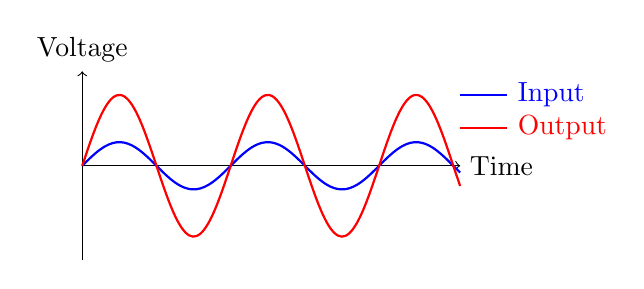
\begin{tikzpicture}[scale=0.6]
            % Grid and axes
            \draw[->] (0,0) -- (8,0) node[right] {Time};
            \draw[->] (0,-2) -- (0,2) node[above] {Voltage};
            
            % Input signal (smaller amplitude)
            \draw[blue, thick, smooth] plot[domain=0:8,samples=100] 
                (\x,{0.5*sin(2*\x r)});
                
            % Output signal (larger amplitude)
            \draw[red, thick, smooth] plot[domain=0:8,samples=100] 
                (\x,{1.5*sin(2*\x r)});
            
            \draw[blue, thick, smooth] (8,1.5) -- (9,1.5) node[right]{Input};
            \draw[red, thick, smooth] (8,0.8) -- (9,0.8) node[right]{Output};
        \end{tikzpicture}
        \caption*{(a) Signal amplification: A small input signal (blue) is amplified to produce a larger output signal (red)}
    \end{minipage}%
    \hfill%
    \begin{minipage}{0.4\textwidth}
        \includegraphics[width=0.3\textwidth]{images/transistor-amplifier.png}
        \caption*{(b) Schematic diagram of a common emitter amplifier circuit}
    \end{minipage}
    \caption{Transistor Power Gain. }
    \label{fig:transistor_power_gain}
\end{figure}

\subsubsection*{Gain: The Measure of Amplification}
Gain is a term that describes how much a device can amplify a signal. It’s usually expressed as a ratio of the output signal to the input signal. For example, if the output signal is 10 times stronger than the input signal, the gain is 10. Gain is a crucial parameter in designing circuits, especially in audio amplifiers and radio receivers.

\subsubsection*{Electrodes of a Bipolar Junction Transistor}
In a BJT, the three electrodes are called the emitter, base, and collector. The emitter is where the electrons start their journey, the base controls the flow, and the collector is where they end up. It’s like a relay race: the emitter hands off the electrons to the base, which then passes them to the collector.

% Diagram labeling the emitter, base, and collector of a bipolar junction transistor.
% \begin{figure}[h!]
%     \centering
%     % \includegraphics[width=0.6\textwidth]{bjt_electrodes.svg}
%     \caption{BJT Electrodes. The diagram labels the emitter, base, and collector of a BJT.}
%     \label{fig:bjt_electrodes}
% \end{figure}

\subsubsection*{Comparison of BJT and FET Transistors}
To wrap things up, let’s compare BJTs and FETs. BJTs are current-controlled devices, while FETs are voltage-controlled. BJTs are generally better for high-power applications, while FETs are more efficient for low-power applications. Both have their strengths and weaknesses, and the choice between them depends on the specific application.

\begin{table}[h!]
    \centering
    \begin{tabular}{|l|l|l|}
        \hline
        \textbf{Characteristic} & \textbf{BJT} & \textbf{FET} \\
        \hline
        Control Mechanism & Current & Voltage \\
        Power Efficiency & Lower & Higher \\
        Input Impedance & Low & High \\
        Typical Use & High-power & Low-power \\
        \hline
    \end{tabular}
    \caption{Comparison of BJT and FET Transistors.}
    \label{tab:bjt_fet_comparison}
\end{table}

\subsubsection{Questions}
\begin{tcolorbox}[colback=gray!10!white,colframe=black!75!black,title={T6B03}]
    Which of these components can be used as an electronic switch?
    \begin{enumerate}[label=\Alph*),noitemsep]
        \item Varistor
        \item Potentiometer
        \item \textbf{Transistor}
        \item Thermistor
    \end{enumerate}
\end{tcolorbox}
A transistor can be used as an electronic switch because it can control the flow of current between two terminals using a small input signal. Varistors, potentiometers, and thermistors do not have this capability.

\begin{tcolorbox}[colback=gray!10!white,colframe=black!75!black,title={T6B04}]
    Which of the following components can consist of three regions of semiconductor material?
    \begin{enumerate}[label=\Alph*),noitemsep]
        \item Alternator
        \item \textbf{Transistor}
        \item Triode
        \item Pentagrid converter
    \end{enumerate}
\end{tcolorbox}
A transistor consists of three regions of semiconductor material: the emitter, base, and collector in a BJT, or the source, gate, and drain in a FET. Alternators, triodes, and pentagrid converters do not have this structure.

\begin{tcolorbox}[colback=gray!10!white,colframe=black!75!black,title={T6B05}]
    What type of transistor has a gate, drain, and source?
    \begin{enumerate}[label=\Alph*),noitemsep]
        \item Varistor
        \item \textbf{Field-effect}
        \item Tesla-effect
        \item Bipolar junction
    \end{enumerate}
\end{tcolorbox}
A Field-Effect Transistor (FET) has a gate, drain, and source. These are the three terminals that control the flow of electrons in a FET. Varistors and BJTs do not have these terminals.

\begin{tcolorbox}[colback=gray!10!white,colframe=black!75!black,title={T6B08}]
    What does the abbreviation FET stand for?
    \begin{enumerate}[label=\Alph*),noitemsep]
        \item Frequency Emission Transmitter
        \item Fast Electron Transistor
        \item Free Electron Transmitter
        \item \textbf{Field Effect Transistor}
    \end{enumerate}
\end{tcolorbox}
FET stands for Field-Effect Transistor. It refers to the way the gate controls the flow of electrons using an electric field.

\begin{tcolorbox}[colback=gray!10!white,colframe=black!75!black,title={T6B10}]
    Which of the following can provide power gain?
    \begin{enumerate}[label=\Alph*),noitemsep]
        \item Transformer
        \item \textbf{Transistor}
        \item Reactor
        \item Resistor
    \end{enumerate}
\end{tcolorbox}
A transistor can provide power gain by amplifying a small input signal to produce a larger output signal. Transformers, reactors, and resistors do not have this capability.

\begin{tcolorbox}[colback=gray!10!white,colframe=black!75!black,title={T6B11}]
    What is the term that describes a device's ability to amplify a signal?
    \begin{enumerate}[label=\Alph*),noitemsep]
        \item \textbf{Gain}
        \item Forward resistance
        \item Forward voltage drop
        \item On resistance
    \end{enumerate}
\end{tcolorbox}
Gain is the term that describes a device's ability to amplify a signal. It is the ratio of the output signal to the input signal.

\begin{tcolorbox}[colback=gray!10!white,colframe=black!75!black,title={T6B12}]
    What are the names of the electrodes of a bipolar junction transistor?
    \begin{enumerate}[label=\Alph*),noitemsep]
        \item Signal, bias, power
        \item \textbf{Emitter, base, collector}
        \item Input, output, supply
        \item Pole one, pole two, output
    \end{enumerate}
\end{tcolorbox}
The electrodes of a bipolar junction transistor are called the emitter, base, and collector. These are the three terminals that control the flow of current in a BJT.

\begin{tcolorbox}[
    colback=gray!10!white,
    colframe=black!75!black,
    title={T6D10},
    sidebyside,
    sidebyside align=top,
    lefthand width=0.45\textwidth
]
What is the function of component 2 in figure T-1?
\begin{enumerate}[label=\Alph*),noitemsep]
    \item Give off light when current flows through it
    \item Supply electrical energy
    \item \textbf{Control the flow of current}
    \item Convert electrical energy into radio waves
\end{enumerate}
\tcblower
\includegraphics[width=0.7\textwidth]{images/t1.png}
\end{tcolorbox}
Component 2 in Figure T-1 is an inductor, which is used to control the flow of current in a circuit. Inductors store energy in a magnetic field and resist changes in current, making them ideal for smoothing out current fluctuations. The other options don’t describe the function of an inductor.
